\documentclass{UoYCSproject}
\usepackage{color,soul}
\usepackage{graphicx}

\addbibresource{refs.bib}

\author{Patrick Buhagiar}
\title{The Impact of Macroeconomic Parameters on Forecasting Financial Markets}
\date{2018-July-06}
\supervisor{Dimitar Kazakov}
\MIP
\wordcount{8832}

\includes{Appendices \ref{cha:usefulpackages}, \ref{cha:gotchas} and
  \ref{cha:deptfac}}

\excludes{\autoref{cha:quoteex}}

\abstract{ 
    Financial forecasting is a common area in machine learning, however a gap in literature was identified with respect to the influence of macroeconomic variables in predicting financial markets. This study attempts to use ensemble methods to predict the direction of the FTSE market in relation to other financial markets and macroeconomic variables in the UK. This study adopts a two-stage process. The first stage consists of creating several ANN models for different time periods that predict the stock market based on the closing prices of other markets. The second stage consists of feeding the results from the first stage and macroeconomic data into another ANN. \hl{TODO add result summary as last sentence}
}

\dedication{To all students everywhere}

\acknowledgements{To my cactus, that I forget to water}
\bibliography{refs}
\begin{document}
\maketitle

\listoffigures
\listoftables

\label{sec:start}
\thispagestyle{empty}\cleardoublepage

\chapter{Introduction}
\label{cha:introduction}



\chapter{Background}
\label{cha:background}

\section{The Relationship Between Macroeconomics and Microeconomics}
Economics can be divided into two branches of study: macroeconomics and microeconomics. Macroeconomics is the study of the behaviour, performance and trends of an economy as a whole \cite{2003economics}. Macro-economists evaluate a variety of economy-wide phenomena such as inflation, gross domestic product (GDP) and unemployment. To keep the economy in check, governments look at these factors to aid in economic policy decision making. Microeconomics on the other hand is the study of how individuals make economic decisions and their effect on the economy. These individuals are classified into consumers, producers and resource owners \cite{dwivedi2002microeconomics}. These individuals interact with the supply and demand for resources while using indications such as interest rates and money as a pricing mechanism for coordination.  Despite being split into two different studies, macroeconomics and microeconomics are deeply interlinked with each other. For example, a stock market's long-run performance is heavily coupled with the economy's performance \cite{davis2008macroeconomic}. This coupled relationship can be seen in \ref{fig:gdpvssp500}. It comes to no surprise that investment analysts focus on economic performance expectations to determine the future prospects of stock markets. The following subsections describe different key factors that fall under macroeconomics and microeconomics.

\begin{figure}[ht]
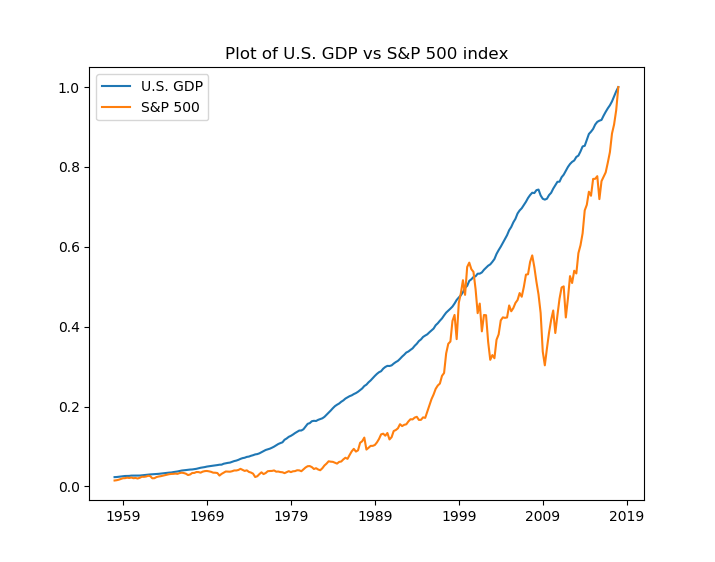
\includegraphics[width=8cm]{GDPvsSP500}
\centering
\caption{Normalised quarterly data from 1958 to 2018 for U.S. GDP and S\&P 500 index. Sources: Standard \& Poor's, U.S. Census Bureau} 
\label{fig:gdpvssp500}
\end{figure}

\subsection{Inflation}


\subsection{Trade Balance}
\subsection{GDP}
\subsection{Unemployment Rate}
\subsection{Interest Rate}

\medskip
 
\printbibliography
\end{document}